\documentclass[10pt,a4paper]{article}
\usepackage{init}
\usepackage{defs}
\usepackage{color}
\usepackage{subcaption}
\newcommand{\red}{\color{red}}
\definecolor{gray}{rgb}{0.4, 0.4, 0.4}

\title{Introduction aux méthodes de Monte Carlo par dynamique Hamiltonienne}
\author{Shmuel RAKOTONIRINA-RICQUEBOURG, Amaury DURAND}
\begin{document}
\maketitle

\begin{abstract}
Ce rapport présente le travail effectué lors d'un projet du cours d'approfondissements en chaînes de Markov par Eric Moulines et Randal Douc dans le cadre du master Mathématiques de l'aléatoire à l'université Paris-Sud. Le contenu exposé ci-dessous repose essentiellement sur \cite{Neal-hmc} et \cite{Douc-mc}. Dans ce rapport, nous présentons l'algorithme Hamiltonian Monte Carlo, un algorithme de type MCMC utilisant une dynamique hamiltonienne pour proposer des mouvements. D'un point de vue théorique, nous nous intéressons à montrer que la loi cible est invariante par le noyau de Markov issu de cet algorithme tout d'abord dans le cas où la dynamique hamiltonienne est simulée de manière exacte puis dans le cas approché. D'un point de vue pratique, nous présentons quelques exemples afin de comparer les performances du Hamiltonian Monte Carlo à celles de l'algorithme classique Random Walk Metropolis. 
\end{abstract}

\tableofcontents
\section{Introduction}
Les méthodes de Monte Carlo par dynamique Hamiltonienne, plus communément appelées Hamiltonian Monte Carlo (HMC), font partie d'une grande famille de méthodes de simulation : les méthodes de Monte Carlo, et plus précisemment de la famille des méthodes de Monte Carlo par chaînes de Markov (ou Monte Carlo Markov Chains, MCMC). Ces méthodes se placent dans le cadre suivant :
\begin{Def}[Carde général]
	Soit $(\xset, \calX)$ un espace mesurable. Soit $\pi$ une loi de probabilité sur cet espace. On suppose que $\pi$ n'est connue qu'à un facteur de proportionnalité près i.e on connait $\lambda \pi$ où $\lambda \in \rset$ une constante. Le but est de pouvoir approcher $\pi f = \EE[f(X)]$ avec $X \sim \pi$ et $f \in \fset_+(\xset, \calX) \cup \fset_b(\xset, \calX)$.
\end{Def}

\subsection{Méthodes de Monte Carlo}

La méthode de Monte Carlo la plus simple (appelée Monte Carlo naïf) est la suivante : supposons que l'on sait simuler des variables aléatoires de loi $\pi$ alors en tirant $n$ échantillons $X_1, \cdots, X_n \siid \pi$, la loi des grands nombre nous indique qu'une bonne approximation de $\pi f$ est $\frac{1}{n} \sum_{i=1}^n f(X_i)$. D'autres méthodes permettent d'atteindre le même but en ne sachant pas simuler de variables aléatoires de loi $\pi$. C'est le cas par exemple de l'échantillonnage d'importance qui consiste à simuler des variables i.i.d sous une loi différente de $\pi$.

Dans ces deux cas, l'approximation de $\pi f$ repose sur une simulation de variables aléatoires i.i.d. Cette particularité permet alors de montrer des résultats de convergence notamment grâce à la loi des grands nombre. Les méthodes de Monte Carlo par chaînes de Markov ne reposent pas sur le caractère i.i.d des variables mais sur les propriétés des Chaînes de Markov. 

\subsection{Monte Carlo Markov Chains (MCMC)}

Les méthodes MCMC se basent sur les notions de loi invariante, de réversibilité et d'ergodicité.

\subsubsection{Loi invariante et réversibilité}

On considère $P$ un noyau de Markov sur $\xset \times \calX$.
\begin{Def}
	Une loi de probabilité $\pi$ sur $(\xset, \calX)$ est dite
	\begin{itemize}
		\item $P$-invariante si $\pi P = \pi$
		\item $P$-réversible si $\forall A,B \in \calX, \pi \otimes P (A \times B) = \pi \otimes P (B \times A)$
	\end{itemize}
\end{Def}

\begin{Prop}
	Toute probabilité $P$-réversible est $P$-invariante.
	% Soit $\pi$ une loi de probabilité sur $(\xset, \calX)$ alors 
	% $$
	% \pi \text{ est } P\text{-reversible} \Rightarrow \pi \text{ est } P\text{-invariante}
	% $$
\end{Prop}

\subsubsection{Ergodicité}

% \begin{Def}[Système ergodique]
%   Soit $(\Omega, \calB, \PP)$ un espace de probabilité. Soit $T : (\Omega, \calB) \to (\Omega, \calB)$ une application mesurable. 
%   \begin{itemize}
%   \item On dit que $\PP$ est invariante pour $T$ si $\forall A \in \calB, \PP[T^{-1}(A)] = \PP[A]$. Dans ce cas, on dit que $(\Omega, \calB, \PP, T)$ est un système dynamique.
%   \item $A \in \calB$ est dit invariant pour $T$ si $A = T^{-1}(A)$.
%   \item Si pour tout $A$ invariant pour $T$ on a $\PP[A] \in \ens{0,1}$ alors on dit que $(\Omega, \calB, \PP, T)$ est un système ergodique. 
%   \end{itemize}
% \end{Def}

% \begin{Thm}\label{thm:ergodic}
%   Soit $P$ un noyau de Markov sur $\xset \times \calX$ et on se place sur l'espace canonique $(\xset^n, \calX^{\otimes n})$. On note $ \theta : \fundef{ \xset^\nset &\to& \xset^\nset \\ (\omega_t)_{t\in \nset} &\mapsto& (\omega_{t+1})_{t \in \nset}}$ et  $\forall k \in \nset^*, \theta_k = \theta_{k-1} \circ \theta$ avec $\theta_0 = \Id$. On suppose
%   \begin{enumerate}
%   \item $P$ possède une loi invariante $\pi$
%   \item $(\xset^\nset, \calX^{\otimes \nset}, \PP_\pi, \theta)$ est ergodique
%   \end{enumerate}
%   Alors pour toute v.a $Y \in L^1(\xset^\nset, \calX^{\otimes \nset}, \PP_\pi)$, pour $\pi$-presque tout $x \in \xset$, 
% $$
%   \frac{1}{n} \sum_{k=0}^{n-1} Y \circ \theta_k \xrightarrow[n \to +\infty]{\PP_x\text{-}\ps} \EE{\pi}[Y]
%   $$
% \end{Thm}

% \begin{Rque}
%   Considérons $(X_k)_{k \in \nset}$ la chaîne de Markov canonique de noyau $P$ et $f \in \fset_+(\xset, \calX) \cup \fset_b(\xset, \calX)$ alors en prenant $Y = f(X_0)$, on a $Y \circ \theta_k = f(X_k)$ et $\EE{\pi}[Y] = \EE{\pi}[f(X_0)] = \pi f$ donc le résultat du théorème \ref{thm:ergodic} se réécrit : pour $\pi$-presque tout $x \in \xset$, 
% $$
%   \frac{1}{n} \sum_{k=0}^{n-1} f(X_k) \xrightarrow[n \to +\infty]{\PP_x\text{-}\ps} \pi f
%   $$
%   Ce qui montre que l'on peut avoir une bonne approximation de $\pi f$ en construisant une chaîne de Markov. De plus il est intéressant de constater que la convergence est $\PP_x$ presque sûre pour $\pi$-presque tout $x \in \xset$ ce qui signifie que quelque soit le point de départ, on est sûr d'avoir une bonne approximation de $\pi f$ si on attend suffisamment longtemps.
% \end{Rque}

\begin{Thm}\label{thm:ergodic}
	Soit $(X_k)_{k \in \nset}$ une chaîne de Markov de noyau $P$ admettant une unique loi invariante $\pi$. Alors pour tout $f \in \fset_+(\xset, \calX) \cup \fset_b(\xset, \calX)$ et pour $\pi$-presque tout $x \in \xset$,
	$$\frac{1}{n} \sum_{k=0}^{n-1} f(X_k) \xrightarrow[n \to +\infty]{\PP_x\text{-}\ps} \pi f$$
\end{Thm}

Les algorithmes MCMC visent à construire, à partir de $\pi$, une chaîne de Markov vérifiant les hypothèses de ce théorème afin d'approcher $\pi f$ par $\frac{1}{n} \sum_{k=0}^{n-1} f(X_k)$.

\subsubsection{Algorithme de Metropolis (Random Walk Metropolis)}

Avant de présenter la méthode HMC, nous définissons ici un autre algorithme MCMC, l'algorithme de Metropolis, que nous utiliserons comme base de comparaison.
%On se place dans le cas où $\xset = \rset^d$ et $\calX = \calB(\rset^d)$. 
On suppose que $\pi$ a une densité $h_\pi$ par rapport à une mesure $\mu$. On considère de plus un loi $Q$ (appelée loi instrumentale) sur $(\xset, \calX)$ symétrique par rapport à $0$ ($Q(A) = Q(-A)$). La construction de la chaîne de Markov se fait en proposant un mouvement (dont l'incrément suit $Q$), puis en acceptant ou en rejetant ce mouvement (algorithme \ref{algo:metropolis}).

\begin{center}
	\begin{algorithm}[H]
		\KwData{$h_\pi$ proportionnel à la densité cible, $Q$ loi simulable}
		$X_0 \leftarrow x \in \xset$ arbitraire\;
		$(U_k)_{k \in \nset} \siid Q$ \;
		\Repeat{une condition d'arrêt}{
			$Y_{k+1} \leftarrow X_k + U_{k+1}$ \tcp*{Proposer un mouvement}
			$\alpha_{k+1} \leftarrow \alpha(X_k, Y_{k+1})$ où $\alpha(x,y) = 1 \wedge \frac{h_{\pi}(y)}{h_\pi(x)}$\;
			$X_{k+1} \leftarrow \piecewise{ Y_{k+1} & \text{avec probabilité } \alpha_{k+1} \\ X_k & \text{avec probabilité } 1 - \alpha_{k+1}}$ \tcp*{Accepter ou rejeter le mouvement}
		}
		\KwRet{$(X_k)_k$}
		\caption{Random Walk Metropolis}
		\label{algo:metropolis}
	\end{algorithm}
\end{center}

Dans cet algorithme, on cherche à explorer l'espace $\xset$ en visitant moins souvent les régions où $h_\pi$ est faible (peu chargées par $\pi$) car ce sont les régions de forte probabilité qui donnent des informations sur la loi $\pi$. Ainsi, si le mouvement proposé vérifie $h_\pi(Y_{k+1}) \geq h_\pi(X_k)$, on se dirige vers une zone plus chargée par $\pi$, on accepte donc le mouvement. Dans le cas contraire, il est moins intéressant de bouger. On autorise quand même le mouvement avec une probabilité $\frac{h_\pi(Y_{k+1})}{h_\pi(X_k)}$ d'autant plus faible que la position proposée est dans une région de probabilité faible.

% \subsubsection{Algorithme de Metropolis-Hastings}

% L'algorithme HMC est une version améliorée de l'algorithme de Metropolis-Hastings. Nous allons donc d'abord définir ce dernier et nous l'utiliserons plus tard comme base de comparaison. On se place dans le cas où $\xset = \rset^d$ et $\calX = \calB(\rset^d)$. 

% On suppose que $\pi$ a une densité $h_\pi$ par rapport à une mesure $\mu$. On considère de plus un noyau markovien $Q$ sur $(\xset, \calX)$ de densité $q$ par rapport à $\mu$. $Q$ est appelé noyau instrumental. La construction de la chaîne de Markov se fait en proposant un mouvement via $Q$, puis en acceptant ou en rejetant ce mouvement (algorithme \ref{algo:metropolis-hastings}).

% \begin{center}
% 	\begin{algorithm}[H]
% 		\KwData{$h_\pi$ proportionnel à la densité cible, $Q$ noyau markovien simulable}
% 		$X_0 \leftarrow x \in \xset$ arbitraire\;
% 		\Repeat{une condition d'arrêt}{
% 			$Y_{k+1} \sim Q(X_k,\cdot)$ \tcp*{Proposer un mouvement}
% 			$\alpha_{k+1} \leftarrow \alpha(X_k, Y_{k+1})$ où $\alpha(x,y) = 1 \wedge \frac{h_{\pi}(y)q(y,x)}{h_\pi(x)q(x,y)}$\;
% 			$X_{k+1} \leftarrow \piecewise{ Y_{k+1} & \text{avec probabilité } \alpha_{k+1} \\ X_k & \text{avec probabilité } 1 - \alpha_{k+1}}$ \tcp*{Accepter ou rejeter le mouvement}
% 		}
% 		\KwRet{$(X_k)_k$}
% 		\caption{Metropolis-Hastings}
% 		\label{algo:metropolis-hastings}
% 	\end{algorithm}
% \end{center}

% Dans cet algorithme, on cherche à explorer l'espace $\xset$ en visitant moins souvent les régions où $h_\pi$ est faible (peu chargées par $\pi$) car ce sont les régions de forte probabilité qui donnent des informations sur la loi $\pi$. Ainsi, si le mouvement proposé vérifie $h_\pi(Y_{k+1})q(Y_{k+1}, X_k) \geq h_\pi(X_k) q(X_k, Y_{k+1})$, on se dirige vers une zone plus chargée par $\pi$, on accepte donc le mouvement. Dans le cas contraire, il est moins intéressant de bouger. On autorise quand même le mouvement avec une probabilité $\frac{h_\pi(Y_{k+1})q(Y_{k+1},X_k)}{h_\pi(X_k)q(X_k,Y_{k+1})}$ d'autant plus faible que la position proposée est dans une région de probabilité faible.

% \begin{Rque}
% 	Il y a d'autres fonctions de rejet $\alpha$ qui permettent à l'algorithme de fonctionner. De même, le choix du noyau $Q$ est un degré de liberté de l'algorithme.

% 	Le choix de $Q$ est en fait une difficulté de l'algorithme, puisque le mouvement proposé doit permettre l'exploration de tout l'espace (afin de passer régulièrement par toutes les régions fortement chargées par $\pi$). Nous verrons que l'algorithme HMC résout ce problème en proposant le mouvement selon une \emph{dynamique hamiltonienne}.
% \end{Rque}

% \begin{Def}
% 	On parle de \emph{Random-walk Metropolis} quand $Q$ est le noyau d'une marche aléatoire
% 	$$Y_{k+1} \leftarrow X_k + U_{k+1}$$
% 	avec $(U_k)_{k \in \nset}$ iid. On supposera que $Q$ admet une densité $q$ par rapport à $\mu$ avec $q(x) = q(-x)$.
% \end{Def}

% \begin{center}
% 	\begin{algorithm}[H]
% 		\KwData{$h_\pi$ proportionnel à la densité cible, $Q$ loi simulable}
% 		$X_0 \leftarrow x \in \xset$ arbitraire\;
% 		$(U_k)_{k \in \nset} \siid Q$ \;
% 		\Repeat{une condition d'arrêt}{
% 			$Y_{k+1} \sim X_k + U_{k+1}$ \tcp*{Proposer un mouvement}
% 			$\alpha_{k+1} \leftarrow \alpha(X_k, Y_{k+1})$ où $\alpha(x,y) = 1 \wedge \frac{h_{\pi}(y)}{h_\pi(x)}$\;
% 			$X_{k+1} \leftarrow \piecewise{ Y_{k+1} & \text{avec probabilité } \alpha_{k+1} \\ X_k & \text{avec probabilité } 1 - \alpha_{k+1}}$ \tcp*{Accepter ou rejeter le mouvement}
% 		}
% 		\KwRet{$(X_k)_k$}
% 		\caption{Random Walk Metropolis}
% 		\label{algo:metropolis}
% 	\end{algorithm}
% \end{center}

\subsection{Principe du Hamiltonian Monte Carlo}

On se place dans le cas où $\xset = \rset^d$, $\calX = \calB(\rset^d)$ et $\mu$ est la mesure de Lebesgue. 
L'algorithme HMC fait partie des algorithmes MCMC, le but est en effet de construire une chaîne de Markov de loi invariante la loi à simuler. Il diffère néanmoins de l'algorithme de Metropolis notamment par le fait que le mouvement proposé suit une \emph{dynamique hamiltonienne} associée à la loi à simuler.

\subsubsection{Dynamique Hamiltonienne}

Un système physique de position $x : \rset_+ \to \rset^d$ et de quantité de mouvement $p : \rset_+ \to \rset^d$ (toutes deux fonctions du temps $t$) est caractérisé par des équations de mouvement de type $\forall t \geq 0, \forall i \in \iseg{1,d}$, 
\begin{equation}\label{eq:hamiltonian-dyn}
	\begin{aligned}
		x_i'(t) &= \frac{\partial H}{\partial p_i} (x(t), p(t)) \\
		p_i' (t) &= -\frac{\partial H}{\partial x_i} (x(t), p(t))
	\end{aligned}
\end{equation}
où $H : \fundef{\rset^d \times \rset^d & \to & \rset \\ (x,p) & \mapsto & H(x,p)}$ s'appelle le {\it hamiltonien} du système, il s'interprète comme une énergie sur $x$ et $p$. En général $H(x,p) = U(x) + K(p)$ où $U$ est l'énergie potentielle et $K$ l'énergie cinétique.

\begin{Rque}\label{rque:edo}
	Les équations \eqref{eq:hamiltonian-dyn} se réécrivent comme une équation différentielle ordinaire d'ordre 1 :
	\begin{equation}\label{eq:edo}
		\forall t \geq 0, \quad z'(t) = F(z(t))
		\tag{EDO}
	\end{equation}
	avec $z : \fundef{ \rset_+ & \to & \rset^{2d} \\ t & \mapsto & [x_1(t), \cdots, x_d(t), p_1(t), \cdots, p_d(t)]^\top}$ et $\forall z \in \rset^{2d}, F(z) = J \nabla H (z)$ où
	$J = \begin{bmatrix}
		0_{d} & I_{d} \\
		-I_{d} & 0_{d}
	\end{bmatrix}$.
	Une solution de \eqref{eq:edo} est dite solution du hamiltonien $H$.
\end{Rque}

\subsubsection{Principe général}

La dynamique hamiltonienne décrit le mouvement d'un objet qui glisse sans frottement le long d'une surface ou d'une courbe. L'objet est décrit par sa position $x \in \rset^d$ et sa quantité de mouvement $p \in \rset^d$ et on lui associe des énergies potentielle $U(x)$ et cinétique $K(p)$.

\begin{Def}[Distribution canonique]
	En physique, une énergie $E : \rset^n \to \rset$ et une température $T > 0$ sont associées à une loi de probabilité par la loi de Boltzmann (ou distribution canonique) de densité par rapport à la mesure de Lebesgue sur $\rset^n$,
	$$\forall x \in \rset^n,  \quad p(x) \propto \exp \left( -\frac{E(x)}{T} \right)$$
\end{Def}


Dans le cas des HMC, on étend l'espace d'états $\xset = \rset^d$ à $\rset^d \times \rset^d$ et on va construire une chaîne de Markov $(Z_k = (X_k, P_k))_{k \in \nset}$ à valeurs dans ce nouvel espace avec $\forall k \in \nset, X_k \indep P_k$ et de loi invariante $\widetilde{\pi} = \pi \otimes \nu$ où $\pi$ est une distribution canonique associée à l'énergie potentielle et $\nu$ est une distribution canonique associée à l'énérgie cinétique. Ainsi leurs densités $h_\pi$ et $h_\nu$ par rapport à la mesure de Lebesgue sur $\rset^d$ vérifient $\forall x \in \rset^d, \forall p \in \rset^d$,
\begin{eqnarray*}
	h_\pi(x) \propto  \exp \left( -\frac{U(x)}{T} \right) & \text{et} &
	h_\nu(p) \propto  \exp \left( -\frac{K(p)}{T} \right)
\end{eqnarray*}

Ce qui donne une loi jointe de densité $h_{\widetilde{\pi}}$ telle que $\forall (x,p) \in \rset^d \times \rset^d$, 
\begin{equation} \label{eq:canonical-dist}
	h_{\widetilde{\pi}}(x,p) \propto \exp \left( -\frac{H(x,p)}{T} \right)
\end{equation}
où le Hamiltonien est défini par $H : (x,p) \mapsto U(x) + K(p)$.

\begin{Rque}
	En dimension 1, on décrit le glissement sans frottement d'un objet sur une rampe. Comme l'énergie potentielle est proportionnelle à la hauteur de la rampe, \eqref{eq:canonical-dist} montre que les creux de la rampe représentent les régions de forte probabilité. L'objet aura tendance à glisser vers les creux de la rampe, mais peut remonter une pente si sa quantité de mouvement $p$ (et donc son énergie cinétique $K(p)$) est assez grande.
\end{Rque}

L'algorithme HMC propose ses mouvements selon le principe suivant : 
\begin{enumerate}
	\item Considérer un objet placé en $X_k$ de quantité de mouvement $P_k$. Cela correspond à l'état $Z_k = (X_k, P_k)$ de l'objet à l'instant $k$.
	\item Tirer une nouvelle quantité de mouvement $\tilde{P}_k \sim \nu$ indépendante de la chaîne et considérer le nouvel état $\tilde{Z}_k = (X_k, \tilde{P}_k)$. 
	\item A partir de l'état $\tilde{Z}_k$, simuler la dynamique hamiltonienne (déterministe) de l'objet pendant une durée fixée.
	\item Considérer $Z_{k+1}^{\rm prop}$ l'état de l'objet à la fin de la simulation, et accepter ou rejeter le mouvement selon une fonction de rejet $\alpha$ dépendant de $H$. 
\end{enumerate}

Il est important de noter que le HMC n'est pas une méthode de Metropolis car, bien que le principe soit similaire (proposer un mouvement et le choisir selon une fonction de rejet dépendant de la loi cible), le HMC tire une nouvelle quantité de mouvement à chaque étape.

Plusieurs problématiques sont alors soulevées : les questions les plus importantes sont de savoir si la loi $\widetilde{\pi}$ est bien invariante et si l'algorithme converge vers cette loi. Nous ne nous intéresserons ici qu'à la question de l'invariance sans résoudre la question de la convergence. De plus, la forme de loi que l'on considère impose des conditions sur les lois $\pi$ et $\nu$, notamment des conditions de régularité de leurs densités (on doit pouvoir dériver le Hamiltonien). Enfin, comment simuler la dynamique hamiltonienne et quelles sont les différences entre le cadre idéal où le mouvement proposé est exactement celui décrit par les équations \eqref{eq:hamiltonian-dyn} et le cadre pratique où l'on doit discrétiser ces équations ?

\paragraph{Hypothèses:}
Afin de pouvoir modéliser le problème par un HMC, on suppose
\begin{equation}\label{eq:hyp}
	\begin{aligned}
		&\mbox{$h_\pi$ et $h_\nu$ sont strictement positives sur $\rset^d$} \\
		&\mbox{$\exists k \geq 1, \ln(h_\pi)$ et $\ln(h_\nu)$ sont de classe $\calC^k$ sur $\rset^d$}\\
		&\mbox{$h_\nu$ est paire} \\
                & H : (x,p) \mapsto U(x) + K(p) \text{ avec } U(x) = - T \ln(h_\pi(x)), K(p) = -T \ln(h_\nu(p))
	\end{aligned}
	\tag{H}
\end{equation}

\begin{Rque}
	La première hypothèse de \eqref{eq:hyp} est nécessaire pour écrire les densités sous la forme canonique. La deuxième permet d'avoir des garanties de régularité des solutions de \eqref{eq:hamiltonian-dyn}. Les deux dernières permettront d'avoir une propriété de réversibilité (proposition \ref{prop:rev}).

	$k \geq 1$ suffit pour tous les résultats énoncés sauf pour les propositions \ref{prop:vol_discret} \ref{prop:rever_discret} où on aura besoin de $k \geq 2$.
\end{Rque}

Nous allons voir que, sous ces hypothèses, dans le cadre idéal (théorique) où l'on a accès aux solutions de \eqref{eq:edo}, le fait de tirer une quantité de mouvement aléatoire puis de suivre la dynamique hamiltonienne laisse la mesure $\tilde{\pi}$ invariante. Dans le cadre où l'on simule la dynamique en discrétisant les équations \eqref{eq:hamiltonian-dyn}, nous verrons que cela n'est plus le cas mais qu'il est alors possible de rendre $\tilde{\pi}$ invariante en incluant le mouvement proposé dans un cadre Metropolis-Hastings (c'est à dire en acceptant le mouvement selon une fonction de rejet). Pour cela, nous avons besoin de quelques propriétés de la dynamique hamiltonienne énoncées dans la section suivante.

%\subsection{Propriétés de l'algorithme}

% Lister les propriétés et bénéfices de HMC en admettant qu'on a les outils de la subsection précédente

\section{Dynamique hamiltonienne}

\subsection{Propriétés de la dynamique hamiltonienne}
\begin{Prop}[conservation du hamiltonien]\label{prop:conservation}
	Le hamiltonien est conservé sur la trajectoire i.e si $z$ est solution de \eqref{eq:edo} alors $H \circ z$ est constant.
\end{Prop}

\begin{proof}
	Remarquons tout d'abord que la matrice $J$ définie dans la remarque \ref{rque:edo} vérifie $\forall u \in \rset^{2d}, \inner{u, Ju} = 0$. Ainsi, si $z$ est solution de \eqref{eq:edo},
	$
	\forall t \in \rset_+, (H \circ z)'(t) = \inner{\nabla H (z(t)), z'(t)} = \inner{\nabla H (z(t)), J \nabla H(z(t))} = 0.
	$
\end{proof}

\begin{Def}[flot hamiltonien]
	On définit le flot du hamiltonien par
	$$
	\forall t \in \rset, \phi_t : \fundef{
		\rset^{2d} & \to & \rset^{2d} \\
		z_0 = (x_0, p_0) &\mapsto & \phi_t(z_0) = (\phi_t^{(1)}(z_0), \phi_t^{(2)}(z_0))
	}
	$$
	où $t \mapsto \phi_t(z_0)$ est l'unique solution de \eqref{eq:edo} avec condition initiale $z(0) = z_0$ (en étendant les solutions à tout $\rset$).
\end{Def}

\begin{Pte}\label{prop:compo}
  $$
  \forall t, s \in \rset, \phi_{t+s} = \phi_t \circ \phi_s.
  $$
\end{Pte}
\begin{proof}
  Soient $s \in \rset$ et $z_0 \in \rset^{2d}$, notons $f : t \mapsto \phi_{t}(z_0)$, $h : t \mapsto t+s$ et $g : t \mapsto \phi_t \circ \phi_s (z_0)$. Alors $f$ et $g$ sont solutions de \eqref{eq:edo} avec conditions initiales $f(0) = z_0$ et $g(0) = \phi_s(z_0)$. De plus $\forall t \in \rset, (f\circ h)'(t) = f'(h(t)) = F(f \circ h(t))$ donc $f \circ h$ est aussi solution de \eqref{eq:edo}. Or $f \circ h (0) = \phi_s(z_0) = g(0)$ donc par unicité de la solution $f \circ h = g$ i.e $\forall t \in \rset, \phi_{t+s}(z_0) = \phi_t \circ \phi_s (z_0)$. 
\end{proof}

\begin{Lem}\label{lem:sol-inverse}
  Soit $z = (x,p)$ une solution de \eqref{eq:edo}. On définit $\bar{z} = (\bar x, \bar p) : \fundef{\rset_{-} & \to & \rset^{2d} \\ t & \mapsto & (x(-t), -p(-t))}$ et $\bar H : \fundef{\rset^{2d} & \to & \rset^{2d} \\ (x,p) & \mapsto & H(x,-p)}$. Alors

  \begin{enumerate}
  \item $\bar{z}$ est solution du hamiltonien $\bar H$ sur $\rset_{-}$ (avec d'autres conditions initiales).
  \item Si $\bar{H} = H$ alors $\forall t \in \rset_+, \phi_t(\bar{z}(-t)) = \bar{z}(0)$
  \end{enumerate}
  
\end{Lem}
\begin{proof}
	%D'une part,
	%$$
	%\forall t \in \rset_-, \bar x'(t) = - x'(-t) = - \frac{\partial H}{\partial p}(x(-t),p(-t)) = - \frac{\partial H}{\partial p}(\bar x(t), - \bar p(t)) = \frac{\partial{\bar H}}{\partial p}(\bar x(t), \bar p(t))
	%$$
	%et d'autre part,
	%$$
	%\forall t \in \rset_-, \bar p'(t) = p'(-t) = - \frac{\partial H}{\partial x}(x(-t),p(-t)) = - \frac{\partial H}{\partial x}(\bar x(t), - \bar p(t)) = - \frac{\partial{\bar H}}{\partial x}(\bar x(t), \bar p(t))
	%$$
	\begin{enumerate}
		\item   Notons $s : z = (x,p) \mapsto (x,-p)$ alors $\forall t \in \rset_-, \bar{z}(t) = s \circ z (-t)$ et $\bar{H} = H \circ s$. De plus
		\begin{equation}\label{eq:ds_dz}
		\forall z \in \rset^{2d}, \frac{ds}{dz}(z) = \begin{bmatrix} I_d & 0_d \\ 0_d & -I_d \end{bmatrix} \doteq S.
		\end{equation}
		Remarquons alors que $S J = - J S$ et $s^{-1} = s$. Ainsi, $\forall y \in \rset^{2d}, \nabla \bar{H} (y) = S \nabla H (s(y))$ et pour $t \in \rset_+$,
		  $$
		  \bar{z}'(t) = - S z'(-t) = - S J \nabla H (z(-t)) = J S \nabla H(z(-t)) =  J \nabla \bar{H} (s^{-1}(z(-t))) = J \nabla \bar{H} (s(z(-t))) = J \nabla \bar{H} (\bar{z}(t)).
		  $$
		% \item Si $\bar{H} = H$, $\bar{z}$ est solution de \eqref{eq:edo} sur $\rset_-$. Notons $f$ l'unique solution de \eqref{eq:edo} sur $\rset$ telle que $f(0) = \bar{z}(-t)$ et $h : u \in \rset \mapsto t + u$. Alors $\forall u \in \rset_+, (f\circ h)'(u) = f(h(u)) = F(f\circ h (u))$ donc $f\circ h$ est solution sur $\rset$. Or $f\circ h (-t) = f(0) = \bar{z}(-t)$ donc par unicité de la solution sur $\rset_-$, $(f \circ h)_{| \rset_-} = \bar{z}$. Cela entraine $f(t) = f \circ h (0) = \bar{z}(0)$. Or par définition de $\phi_t$ et unicité de la solution sur $\rset_+$, on a $f_{|\rset_+} : u \in \rset_+ \mapsto \phi_u(\bar{z}(-t))$ donc pour $u = t$ on obtient $\phi_t(\bar{z}(-t)) = f(t) = \bar{z}(0)$
		\item Si $\bar{H} = H$, $\bar{z}$ est solution de \eqref{eq:edo} sur $\rset_-$ donc $\forall t \in \rset_+, \bar z(-t) = \phi_{-t}(\bar z(0))$ donc $\phi_t(\bar{z}(-t)) = \phi_0(\bar{z}(0)) = \bar{z}(0)$
	\end{enumerate}
\end{proof}

\begin{Rque}\label{rque:Hbar}
	Sous les hypothèses \eqref{eq:hyp}, la parité de $h_\nu$ donne la parité de $K$. Comme $H(x,p) = U(x)+K(p)$, on en déduit $H = \bar H$.
\end{Rque}

\begin{Prop}[réversibilité]\label{prop:rev}
	On se place sous les hypothèses \eqref{eq:hyp}. Alors pour tout $t \in \rset_+, \phi_t$ est un $\calC^k$-différomorphisme et
	$$
	\phi_t^{-1} : (x,p) \mapsto (\phi_t^{(1)}(x, -p), - \phi_t^{(2)}(x, -p))
	$$
\end{Prop}
\begin{proof}
	$\phi_t$ est $\calC^k$ comme flot d'une équation différentielle $\calC^k$. Si on admet la formule de l'inverse, on y lit que $\phi_t^{-1}$ est $\calC^k$. Il suffit donc de montrer cette formule.

	Fixons $t \in \rset_+$ et $(x_0,p_0) \in \rset^{2d}$. Notons $z=(x,p)$ la solution sur $\rset_+$ de \eqref{eq:edo} avec $z(0) = (x_0,p_0)$ et notons
	$$
	\bar \phi_t : (x,p) \mapsto (\phi_t^{(1)}(x, -p), - \phi_t^{(2)}(x, -p))
	$$
        \begin{itemize}
		\item D'une part,
		$$
		\bar \phi_t(\phi_t(x_0,p_0)) = \bar \phi_t(z(t)) = (\phi_t^{(1)}(\bar z(-t)), - \phi_t^{(2)}(\bar z(-t))) \overset{\text{(lemme \ref{lem:sol-inverse})}}{=} (x_0, p_0)
		$$
		car $\bar z(0) = (x_0,-p_0)$.
		%Par lemme \ref{lem:sol-inverse} et remarque \ref{rque:Hbar}, $\bar z$ est solution sur $\rset_-$ de \eqref{eq:edo} avec $\bar z(0) = (x_0,-p_0)$ donc
		%$$
		%\phi_t^{(1)}(\bar z(-t)) = x_0, \phi_t^{(2)}(\bar z(-t)) = -p_0
		%$$
		%ce qui donne que $\bar \phi_t(\phi_t(x_0,p_0)) = (x_0,p_0)$.

		\item D'autre part,
		$$
		\bar \phi_t(x_0,-p_0) = (\phi_t^{(1)}(x_0, p_0), - \phi_t^{(2)}(x_0, p_0)) = (x(t),-p(t)) = \bar z(-t)
		$$
		donc
		$$
		\phi_t (\bar \phi_t(x_0,-p_0)) = \phi_t(\bar z(-t)) = \bar{z}(0) = (x_0,-p_0).
		$$
	\end{itemize}
	Ceci étant vrai pour tout $(x_0,p_0)$, on a donc $\bar \phi_t = \phi_t^{-1}$.
\end{proof}


\begin{Prop}[conservation du volume]\label{prop:vol}
	La dynamique hamiltonienne conserve le volume, au sens où
	$$
	\forall t \in \rset_+, \forall z \in \rset^{2d}, \detjacob{\phi_t}{z} = 1.
	$$
\end{Prop}
\begin{proof}
On ne donnera pas de preuve détaillée de cette proposition, mais la preuve repose sur le caractère simplectique lié à la remarque \ref{rque:edo}.
\end{proof}

\subsection{Discrétisation des équations}

% Donner rapidement les résultats déterministes de l'article sur l'hamiltonnien (2.1 et 2.2 de l'article), peut-être qu'on peut se contenter du cas U = -log(h_\pi) et K = \norm{v}/2 (T = 1, m = 1)
% Expliquer la méthode du saute-mouton pour simuler la dynamique hamiltonienne, en quoi elle est meilleure, en quoi elle peut-être simplifiée (2.3 de l'article), éventuellement en quoi elle "conserve le volume"


%\begin{center}
%        \begin{algorithm}[H]
%        	\KwData{pas $\epsilon$, nombre de pas $L$, état initial $(x_0,p_0)$}
%        	$(x,p) \leftarrow (x_0,p_0)$\;
%        	$p \leftarrow p - \frac{\epsilon}{2} \nabla U(x)$ \tcp*{Demi-pas en $p$}
%        	\For(\tcp*[h]{Saute-mouton}){$k \in \llbracket 1,L-1 \rrbracket$}{
%        		$x \leftarrow x + \epsilon p$\;
%        		$p \leftarrow p - \epsilon \nabla U(x)$\;
%        	}
%        	$x \leftarrow x + \epsilon p$ \tcp*{Dernier pas en $x$}
%        	$p \leftarrow p - \frac{\epsilon}{2} \nabla U(x)$ \tcp*{Demi-pas en $p$}
%        	\KwRet{$(x,p)$}
%        	\caption{Discrétisation de l'évolution par saute-mouton (\emph{leapfrog})}
%        	\label{algo:leapfrog}
%        \end{algorithm}
%\end{center}

\begin{center}
	\begin{algorithm}[H]
		\KwData{pas $\epsilon$, nombre de pas $L$, état initial $(x_0,p_0)$}
		\For(\tcp*[h]{Saute-mouton}){$k \in \llbracket 0, L-1 \rrbracket$}{
			$x_{k+1} \leftarrow x_k + \epsilon \nabla K \left( p_k - \frac{\epsilon}{2} \nabla U(x_k) \right)$\;
			$p_{k+1} \leftarrow p_k - \frac{\epsilon}{2} \nabla U(x_k) - \frac{\epsilon}{2} \nabla U(x_{k+1})$\;
		}
		\KwRet{$(x_L,p_L)$}
		\caption{Discrétisation de l'évolution par saute-mouton (\emph{leapfrog})}
		\label{algo:leapfrog}
	\end{algorithm}
\end{center}

\begin{Def}[flot approché] \label{def:flot_approche}
	Soient $\epsilon > 0$ et $L \in \nset^*$, on définit le flot approché du hamiltonien par $L$ itérations de l'algorithme leapfrog par $\hat{\phi}_L = \hat{\phi}^L$ où 
	$$
	\hat{\phi} : \fundef{\rset^{2d} & \to & \rset^{2d} \\
	z = (x, p) & \mapsto & (\hat{\phi}^{(1)}(z), \hat{\phi}^{(2)}(z))
	}
	$$
	avec
	\begin{align*}
	\hat{\phi}^{(1)} : (x,p) & \mapsto x + \epsilon \nabla K \left( p - \frac{\epsilon}{2} \nabla U(x) \right) \\
	\hat{\phi}^{(2)} : (x,p) & \mapsto p - \frac{\epsilon}{2} \nabla U(x) - \frac{\epsilon}{2} \nabla U(\hat{\phi}^{(1)}(x,p))
	\end{align*}
\end{Def}

La proposition \ref{prop:vol_discret} est l'analogue de la proposition \ref{prop:vol} mais pour le flot approché.

\begin{Prop}[conservation du volume]\label{prop:vol_discret}	
	Sous les hypothèses \eqref{eq:hyp} avec $k \geq 2$ ($U$ et $K$ de classe $\calC^2$), la discrétisation de la dynamique hamiltonienne par l'algorithme leapfrog conserve le volume, au sens où
	$$
	\forall z \in \rset^{2d}, \detjacob{\hat \phi}{z} = 1.
	$$
\end{Prop}
\begin{proof}
	$\hat \phi$ conserve le volume comme composée de cisaillements (qui préservent le volume). Plus précisément, la définition \ref{def:flot_approche} peut s'écrire $\hat \phi= \varphi_p \circ \varphi_x \circ \varphi_p$ où
	$$
	\varphi_x : \fundef{
		\rset^{2d} & \to & \rset^{2d} \\
		(x,p) & \mapsto & (x + \epsilon \nabla K(p),p)
	}
	\text{ et }
	\varphi_p : \fundef{
		\rset^{2d} & \to & \rset^{2d} \\
		(x,p) & \mapsto & (x,p - \frac \epsilon 2 \nabla U(x))
	}
	$$
	$U$ et $K$ étant $calC^2$, on a les jacobiennes
	$$
	\frac{d\varphi_x}{dz}(x,p) =
	\begin{bmatrix}
	I_d & \epsilon \frac{d\nabla K}{dp}(p) \\
	0 & I_d
	\end{bmatrix}
	\text{ et }
	\frac{d\varphi_p}{dz}(x,p) =
	\begin{bmatrix}
	I_d & 0 \\
	- \frac \epsilon 2 \frac{d\nabla U}{dx}(x) & I_d
	\end{bmatrix}
	$$
	qui sont bien de déterminant $1$ en tout point ($I_d$ désigne la matrice identité de taille $d$). Ainsi, pour $z \in \rset^{2d}$,
	$$
	\detjacob{\hat \phi}{z} = \detjacob{\varphi_p}{\varphi_x(\varphi_p(z))} \detjacob{\varphi_x}{\varphi_p(z)} \detjacob{\varphi_p}{z} = 1.
	$$
\end{proof}

\begin{Prop}[réversibilité]\label{prop:rev-leapfrog}
  Sous les hypothèses \eqref{eq:hyp}, $\hat{\phi}$ est inversible avec $\hat{\phi}^{-1} : (x,p) \mapsto (\hat{\phi}^{(1)}(x,-p), -\hat{\phi}^{(2)}(x,-p))$, ce qui entraîne $\forall L \in \nset^*, \hat{\phi}_L$ est inversible avec $\hat{\phi}_L^{-1} : (x,p) \mapsto (\hat{\phi}_L^{(1)}(x,-p), -\hat{\phi}_L^{(2)}(x,-p))$. 
\end{Prop}
\begin{proof}
	Notons $\bar{\phi} : (x,p) \mapsto (\hat{\phi}^{(1)}(x,-p), -\hat{\phi}^{(2)}(x,-p))$, ainsi $\bar \phi = s \circ \hat \phi \circ s$ avec $s : (x, p) \mapsto (x,-p)$. Alors
	\begin{itemize}
		\item Soient $x,p \in \rset^d$. Notons $(\tilde x, \tilde p) = \hat \phi(x,-p)$ de sorte que $\bar \phi(x,p) = (\tilde x, - \tilde p)$
		\begin{align*}
			\hat{\phi}^{(1)} (\bar{\phi}(x,p))
			&= \tilde x + \epsilon \nabla K \left( -\tilde p - \frac{\epsilon}{2} \nabla U (\tilde x) \right) \\
			&= x + \epsilon \nabla K \left(-p - \frac{\epsilon}{2} \nabla U(x) \right) + \epsilon \nabla K \left(p + \frac{\epsilon}{2} \nabla U(x) + \frac{\epsilon}{2} \nabla U(\tilde x) - \frac{\epsilon}{2} \nabla U (\tilde x) \right) \\
			&= x + \epsilon \nabla K \left(-p - \frac{\epsilon}{2} \nabla U(x) \right) + \epsilon \nabla K \left(p + \frac{\epsilon}{2} \nabla U(x)\right) \\
			&= x \text{ car sous \eqref{eq:hyp}, } K \text{ est paire donc } \nabla K \text{ est impaire.}
		\end{align*}

		De plus
		\begin{align*}
			\hat{\phi}^{(2)}(\bar{\phi}(x,p))
			&= -\tilde p - \frac{\epsilon}{2} \nabla U(\tilde x) - \frac{\epsilon}{2} \nabla U(\hat{\phi}^{(1)}(\bar{\phi}(x,p))) \\
			&= p + \frac{\epsilon}{2} \nabla U(x) + \frac{\epsilon}{2} \nabla U(\tilde x) - \frac{\epsilon}{2} \nabla U(\tilde x) - \frac{\epsilon}{2} \nabla U(x) \\
			&= p
		\end{align*}
		Donc $\hat{\phi} \circ \bar{\phi} = \Id$
		% \item Soient $x,p \in \rset^d$, 
		%   $$
		%   \bar{\phi}^{(1)} (\hat{\phi}(x,p)) = \hat{\phi}^{(1)} (\bar{\phi}(x,-p)) = x 
		%   $$
		%   et
		%   $$
		%   \bar{\phi}^{(2)} (\hat{\phi}(x,p)) = - \hat{\phi}^{(1)} (\bar{\phi}(x,-p)) = -(-p) = p
		%   $$

		%     Donc $\bar{\phi} \circ \hat{\phi} = \Id$
		%   \end{itemize}
		%   Ainsi $\hat{\phi}^{-1} = \bar{\phi}$
		\item On a donc
		$\Id = \hat \phi \circ \bar \phi = \hat \phi \circ s \circ \hat \phi \circ s.$
		En composant à gauche et à droite par $s$, on obtient
		$s^2 = s \circ \hat \phi \circ s \circ \hat \phi \circ s^2$.
		Soit, en utilisant $s^2 = \Id$,
		$\Id = s \circ \hat \phi \circ s \circ \hat \phi.$
	\end{itemize}
	Ainsi $\hat{\phi}^{-1} = \bar{\phi}$
\end{proof}

%\begin{Prop}\label{prop:leapfrog}
%  Soient $\epsilon > 0, L \in \nset^*$ et $(x_0, p_0) \in \rset^{d} \times \rset^{d}$. Alors les positions et quantité de mouvement obtenues par l'algorithme leapfrog vérifient
%  \begin{align*}
%    x_L &= x_0 + \epsilon \sum_{i=0}^{L-1} \nabla K \left( p_i - \frac{\epsilon}{2} \nabla U(x_i) \right) \\
%    p_L &= p_0 - \frac{\epsilon}{2} \nabla U(x_0) - \epsilon \sum_{i=1}^{L-1} \nabla U(x_i) - \frac{\epsilon}{2} \nabla U(x_L) 
%  \end{align*}
%  %et dans le cas particulier où $K : p \mapsto \frac{p^\top p }{2}$
%\end{Prop}      

\section{Hamiltonian Monte-Carlo}

\subsection{Cas idéal : solution exacte de la dynamique hamiltonienne}

Dans le cas idéal où l'on a accès à une solution exacte de la dynamique hamiltonienne, i.e. si l'on connait le flot $\phi_t$ pour tout $t \in \rset_+$, la stratégie proposée est de suivre le flot à chaque étape après avoir tiré aléatoirement une quantité de mouvement.

\begin{center}
	\begin{algorithm}[H]
		\KwData{$h_\pi$ proportionnel à la densité cible, $t$ une durée sur laquelle suivre la dynamique}
		$X_0 \leftarrow x \in \xset$ arbitraire\;
		\Repeat{une condition d'arrêt}{
			$\tilde{P}_k \sim \mathcal \nu$ et $\tilde{P}_k \indep (Z_0, \cdots, Z_{k})$ \tcp*{Tirer la quantité de mouvement}
			$\tilde{Z}_k \leftarrow (X_k, \tilde{P}_k)$ \;
			$Z_{k+1} = (X_{k+1}, P_{k+1}) \leftarrow \phi_t(\tilde{Z}_k)$ \tcp*{Suivre la dynamique}
		}
		\KwRet{$(X_k)_k$}
		\caption{Hamiltonian Monte-Carlo, cas idéal}
		\label{algo:HMC-ideal}
	\end{algorithm}
\end{center}

\begin{Def}[semi-groupe Markovien]
	Une famille $(R_t)_{t \in \rset_+}$ de noyaux de Markov est un semi-groupe Markovien si $\forall t,s \in \rset_+, R_{t+s} = R_t R_s$
\end{Def}

\begin{Prop}[invariance de la loi]\label{prop:inv-ideal}
	On se place sous les hypothèses \eqref{eq:hyp}. Alors

	\begin{enumerate}
		\item Pour $t \in \rset_+$, le processus $(Z_k)_{k \in \nset}$ défini par l'algorithme \ref{algo:HMC-ideal} est une chaîne de Markov homogène de noyau $QR_t$ sur $\rset^{2d}$ avec
		% $$
		% Q : \fundef{
		% \rset^{2d} \times \calB(\rset^{2d}) & \to & [0,1] \\
		% ((x,p), A) & \mapsto & \delta_x \otimes \nu(A)
		% }
		% $$
		% $$
		% P_t : \fundef{
		% \rset^{2d} \times \calB(\rset^{2d}) & \to & [0,1] \\
		% (z, A) & \mapsto & \delta_{\phi_t(z)}(A) = \ind_A(\phi_t(z))
		% }
		% $$
		$$
		Q((x,p),\cdot) = \delta_x \otimes \nu
		$$
		$$
		R_t((x,p),\cdot) = \delta_{\phi_t(z)}
		$$
		\item $(R_t)_{t \in \rset_+}$ est un semi-groupe Markovien.
		\item Pour tout $t \in \rset_+$, $\widetilde{\pi}$ est $QR_t$-invariante. 
	\end{enumerate}
\end{Prop}
\begin{proof}
	\begin{enumerate}
		\item On note $(\calF_k)_{k \in \nset} = (\sigma(Z_j, j\leq k))_{k \in \nset}$ la filtration canonique associée à $Z$. Soit $A \in \calB(\rset^{2d})$ alors $\PP[Z_{k+1} \in A \given{\calF_k}] = \PP[\phi_t(X_k, \tilde{P}_k) \in A \given{\calF_k}] = \PP[\phi_t(X_k, \tilde{P}_k) \in A \given{\calF_k}]$. Comme $\tilde{P}_k \indep \calF_k$, on a donc $\PP[Z_{k+1} \in A \given{\calF_k}] = \hat{F}(X_k)$ où $\forall x \in \rset^d, \hat{F}(x) = \PP[\phi_t(x, \tilde{P}_1) \in A]$. Ainsi $(Z_k)_{k \in \nset}$ est une chaîne de Markov homogène de noyau $N$ tel que
		$$
		\forall (x,p) \in \rset^{2d}, \forall A \in \calB(\rset^{2d}), N((x,p), A) = \PP[\phi_t(x, \tilde{P}_1) \in A] = \int \ind_A(\phi_t(x, p_1)) \nu(dp_1).
		$$
		Or
		$$
		Q R_t((x,p),A) = \int Q((x,p), dx_1dp_1) R_t((x_1, p_1), A) = \int \delta_x(dx_1) \nu(dp_1) \ind_A(\phi_t(x_1, p_1)) = \int \ind_A(\phi_t(x,p_1)) \nu(dp_1).
		$$
		Donc $(Z_k)_{k \in \nset}$ est une chaîne de Markov homogène de noyau $QR_t$.

		\item Soient $t,s \in \rset_+$, $z \in \rset^{2d}$ et $A \in \calB(\rset^{2d})$. Alors
                  \begin{multline*}
                    R_t R_s (z, A) = \int R_t(z, dz_1) R_s(z_1, A) = \int \delta_{\phi_t(z)}(dz_1) \ind_A(\phi_s(z_1)) = \ind_A(\phi_s \circ \phi_t(z)) = \ind_A(\phi_{s+t}(z)) = R_{s+t}(z,A) \\ = R_{t+s}(z,A)
                  \end{multline*}

		\item Montrons que $\widetilde{\pi}$ est $Q$ et $R_t$ invariante (elle sera donc $QR_t$-invariante). Soit $A \in \calB(\rset^{2d})$, alors
		$$
		\widetilde{\pi} Q (A) = \int \pi(dx) \nu(dp) \delta_x(dx_1) \nu(dp_1) \ind_A(x_1, p_1) = \int \pi(dx) \nu(dp_1) \ind_A(x, p_1) = \int \widetilde{\pi}(dxdp_1) \ind_A(x, p_1) = \widetilde{\pi}(A) 
		$$

		Soient $t \in \rset_+$ et $A \in \calB(\rset^{2d})$, alors
		\begin{align*}
		\widetilde{\pi} R_t (A)
		&= \int \widetilde{\pi}(dz) R_t(z, A) \\
		&\propto \int \exp \left(-\frac{H(z)}{T} \right) \ind_A(\phi_t(z)) dz\\
		&\overset{(*)}{=} \int \exp \left(-\frac{H \circ \phi_t^{-1}(y)}{T} \right) \ind_A(y) dy \\
		&\overset{(**)}{=} \int \exp \left(-\frac{H(y)}{T} \right) \ind_A(y) dy \\
		&= \widetilde{\pi}(A).
		\end{align*}
		$(*)$ : en faisant le changement de variable $y = \phi_t(z)$ comme $\phi_t$ est un $\calC^1$ difféomorphisme (proposition \ref{prop:rev}) de jacobien égal à $1$ (proposition \ref{prop:vol}) \\
		$(**)$ : par la proposition \ref{prop:conservation} on sait que $H \circ \phi_t = H$. De plus sous les hypothèses \eqref{eq:hyp}, $\bar{H} = H \circ s = H$ où $s : (x,p) \mapsto (x, -p)$. Ainsi $H \circ \phi_t^{-1} = H \circ s \circ \phi_t \circ s = H \circ \phi_t \circ s = H \circ s = H$ 
	\end{enumerate}
\end{proof}


\subsection{Cas concret : solution approchée de la dynamique hamiltonienne}
Dans le cas où l'on n'a pas accès aux solutions exactes de \eqref{eq:edo}, on utilise le flot appoché $\hat{\phi}_L$. La première idée serait de simplement remplacer $\phi_t$ par $g \circ \hat{\phi}_L$ dans l'algorithme \ref{algo:HMC-ideal} où $g : \rset^{2d} \to \rset^{2d}$ est une fonction à déterminer. On obtient donc des noyaux $Q$ (défini en proposition \ref{prop:inv-ideal}) et
$$
\hat{R}_L : \fundef{
  \rset^{2d} \times \calB(\rset^{2d}) & \to & [0,1] \\
  (z, A) & \mapsto & \delta_{g \circ \hat{\phi}_L(z)}(A)
}
$$
$\widetilde{\pi}$ est toujours $Q$-invariante mais n'est plus forcément $\hat{R}_L$-invariante car après la discrétisation, on n'a plus la propriété de conservation du hamiltonien. Néanmoins la proposition suivante montre que pour un bon choix de $g$, il est possible d'utiliser le mouvement proposé dans un algorithme de Metropolis.

\begin{Prop}[réversibilité]\label{prop:rever_discret}
	Sous les hypothèses \eqref{eq:hyp} avec $k \geq 2$ ($U$ et $R$ de classe $\calC^2$), on considère $g = s : (x, p) \mapsto (x,-p)$ et on définit
	$$
	\alpha : \fundef{
	\rset^{2d} \times \rset^{2d} & \to & [0,1] \\
	(z_0, z_1) & \mapsto & 1 \wedge \exp(\frac{-H(z_1)+H(z_0)}{T})
	}
	$$
	et on note $\hat{R}_L^\alpha$ le noyau de Metropolis-Hasting associé au noyau instrumental $\hat{R}_L$ et à la fonction de rejet $\alpha$. Alors $\widetilde \pi$ est $\hat{R}_L^\alpha$-réversible (et donc $\hat{R}_L^\alpha$-invariant). 
\end{Prop}
\begin{proof}
	Notons $\psi_L = s \circ \hat \phi_L$, de sorte que $\hat{R}_L(z,\cdot) = \delta_{\psi_L(z)}$. Ainsi,
	$$
	\hat{R}_L^\alpha(z,A) = \alpha(z,\psi_L(z)) \ind_A(\psi_L(z)) + (1-\alpha(z,\psi_L(z))) \ind_A(z)
	$$
	et pour $A,B$ boréliens,
	$$
	\widetilde \pi \otimes \hat{R}_L^\alpha (A \times B)
	=
	\int \ind_A(z) \hat{R}_L^\alpha(z,B) e^{-H(z)/T} dz
	=
	\Lambda_1(A,B) + \Lambda_2(A,B)
	$$
	où
	$$
	\Lambda_1(A,B) = \int \ind_A(z) \ind_B(\psi_L(z)) \alpha(z,\psi_L(z)) e^{-H(z)/T} dz
	$$
	et
	$$
	\Lambda_2(A,B) = \int \ind_A(z) \ind_B(z) (1-\alpha(z,\psi_L(z))) e^{-H(z)/T} dz.
	$$
	Il suffit, pour avoir la $\hat{R}_L^\alpha$-réversibilité, que les expressions $\Lambda_1(A,B)$ et $\Lambda_2(A,B)$ soient toutes les deux symétriques en $A$ et $B$. C'est le cas pour $\Lambda_2$, reste à étudier $\Lambda_1$.

	D'après l'expression définissant $\alpha$, on a $\alpha(z_0,z_1) e^{-H(z_0)/T} = e^{-H(z_0)/T} \wedge e^{-H(z_1)/T}$, donc
	\begin{equation}\label{eq:Lambda1}
	\Lambda_1(A,B) = \int \ind_A(z) \ind_B(\psi_L(z)) \left( e^{-H(z)/T} \wedge e^{-H(\psi_L(z))/T} \right) dz
	\end{equation}

	On cherche à faire un changement de variable $z \mapsto \psi_L(z)$. Par proposition \ref{prop:rev-leapfrog}, on a $(\psi_L)^{-1} = \psi_L$. $U$ et $K$ sont de classe $\calC^2$ par hypothèse donc $\hat \phi$ est, par définition \ref{def:flot_approche}, de classe $\calC^1$. Comme $(\psi_L)^{-1} = \psi_L = s \circ \hat \phi^L$, $\psi_L$ est donc un $\calC^1$-difféomorphisme. De plus, $s$ oppose le volume ($\detjacob{s}{z} = -1$ par équation \eqref{eq:ds_dz}) et $\hat \phi$ conserve le volume (par proposition \ref{prop:vol_discret}), donc $\psi_L$ aussi :
	$$
	\forall z \in \rset^{2d}, \detjacob{\psi_L}{z} = \detjacob{s}{\hat \phi^L(z)} \detjacob{\hat \phi^L}{z} = -1.
	$$

	Ainsi, le changement de variable dans \eqref{eq:Lambda1} donne
	$$
	\Lambda_1(A,B) = \int \ind_A(\psi_L(z)) \ind_B(z) \left( e^{-H(z)/T} \wedge e^{-H(\psi_L(z))/T} \right) dz = \Lambda_1(B,A).
	$$

	Ainsi, $\Lambda_1$ et $\Lambda_2$ sont bien symétriques en $A$ et $B$, donc $\widetilde \pi \otimes \hat{R}_L^\alpha (A \times B) = \widetilde \pi \otimes \hat{R}_L^\alpha (B \times A)$ : $\widetilde \pi$ est $\hat{R}_L^\alpha$-réversible.
\end{proof}
L'algorithme qui découle de ces propriétés est le suivant :



\begin{center}
	\begin{algorithm}[H]
		\KwData{$h_\pi$ proportionnel à la densité cible, $\epsilon$ pas du saute-mouton, $L$ nombre de pas du saute-mouton}
		$X_0 \leftarrow x \in \xset$ arbitraire\;
		\Repeat{une condition d'arrêt}{
			$\tilde{P}_k \sim \mathcal \nu$ et $\tilde{P}_k \indep (Z_0, \cdots, Z_{k})$ \tcp*{Tirer la quantité de mouvement}
			$\tilde{Z}_k \leftarrow (X_k, \tilde{P}_k)$ \;
			$Z_{k+1}^{\rm prop} = (X_{k+1}^{\rm prop}, P_{k+1}^{\rm prop}) \leftarrow s \circ \hat{\phi}_L(\tilde{Z}_k)$ \tcp*{Suivre la dynamique approchée} 
                        $\alpha_{k+1} \leftarrow 1 \wedge \exp \left( \frac{- H(Z_{k+1}^{\rm prop}) + H(\tilde{Z}_k) }{T} \right)$ \;

                        $Z_{k+1} \leftarrow \piecewise{ Z_{k+1}^{\rm prop} & \text{avec probabilité } \alpha_{k+1} \\ \tilde{Z}_k & \text{avec probabilité } 1 - \alpha_{k+1}}$ \tcp*{Accepter ou rejeter le mouvement}
		}
		\KwRet{$(X_k)_k$}
		\caption{Hamiltonian Monte-Carlo, cas concret}
		\label{algo:HMC}
	\end{algorithm}
\end{center}


%\begin{center}
%        \begin{algorithm}[H]
%        	\KwData{$h_\pi$ proportionnel à la densité cible, $\epsilon$ pas du saute-mouton, $L$ nombre de pas du saute-mouton}
%        	$X_0 \leftarrow x \in \xset$ arbitraire\;
%        	\Repeat{une condition d'arrêt}{
%        		$P_k \sim \mathcal N(0,1)$\tcp*{Tirer la quantité de mouvement}
%        		$(X_{prop},P_{prop}) \leftarrow \texttt{leapfrog}(X_k,P_k)$\tcp*{Proposer un mouvement}
%        		$U_k \leftarrow U(X_k)$\;
%        		$K_k \leftarrow \norm{P_k}^2/2$\;
%        		$U_{prop} \leftarrow U(X_{prop})$\;
%        		$K_{prop} \leftarrow \norm{P_{prop}}^2/2$\;
%        		\eIf{$\mathcal U([0,1]) < \exp(U_k-U_{prop}+K_k-K_{prop})$}{
%        			$X_{k+1} \leftarrow X_{prop}$ \tcp*{Accepter}
%        		}{
%        			$X_{k+1} \leftarrow X_k$ \tcp*{Rejeter}
%        		}
%        	}
%        	\KwRet{$(X_k)_k$}
%        	\caption{Hamiltonian Monte-Carlo}
%        	\label{algo:HMC}
%        \end{algorithm}
%\end{center}


\section{Simulations}
Nous montrons dans cette section quelques résultats obtenus en pratique avec les deux algorithmes Random-walk Metropolis (RWM) et Hamiltonian Monte Carlo (HMC). Dans tous les exemples suivants, $T = 1$ et l'énergie cinétique est définie pas $K : p \mapsto \frac{\norm{p}^2}{2}$ ce qui correspond à une énergie cinétique courante en physique et donne une loi $\nu$ normale centrée réduite. Nous allons tester trois lois $\pi$ à simuler : une normale, un mélange de gaussienne et une loi bayesian lasso. Les hypothèses \eqref{eq:hyp} sont vérifiées avec $k = 2$ dans les deux premiers cas mais pas dans le dernier (car $h_\pi$ n'est pas différentiable en 0). Afin de comparer les deux algorithmes, nous allons étudier leur comportement lorsque le point de départ $(X_0)$ change (le théorème \ref{thm:ergodic} permet d'avoir convergence quel que soit le point de départ mais cette convergence peut s'avérer plus lente si celui-ci est dans une portion de l'espace correspondant à la queue de la densité cible). Nous allons de plus analyser l'autocorrelation du processus $(X_t)_{t \in \nset}$ car elle rend compte de la stationnarité (approchée) du processus.

\paragraph{Paramètres communs à toutes les simulations :}
Pour toutes les simulations, on prend $\epsilon = 0.1$, $L = 25$ ou $L \sim \calU(\iseg{1,25})$ (à chaque itération), les algorithmes ont été lancés sur $200\,000$ itérations. Les autocorrelations sont calculées sur la première coordonnée de $X_k$ pour $k \geq 100\,000$ et on ne regarde que les $50$ premières composantes des autocorrelations.

\subsection{Test sur une loi normale}
On considère ici $\pi = \calN\left(\begin{bmatrix} 0 \\ 0 \end{bmatrix}, \begin{bmatrix} 0.4 & 0.2 \\ 0.2 & 0.4  \end{bmatrix} \right)$.

La figure \ref{fig:normal} montre que l'algorithme HMC a bien tendance à suivre une dynamique plus cohérente par rapport à l'énergie potentielle $U$ (et donc la loi $\pi$). La trajectoire obtenue semble mieux rendre compte de la corrélation entre les deux coordonnées. Bien que le HMC avec $L$ constant semble mieux suivre la dynamique, notons que le fait de randomiser $L$ permet un gain en stationnarité. En effet, la figure \ref{fig:normal_autocor} montre que si on prend $L$ constant, les autocorrelations oscillent et restent assez fortes. Cela peut s'expliquer facilement en se rappellant l'interprétation physique du HMC : on simule le mouvement d'un objet sur une surface. Cet objet aura donc tendance à effectuer des allez-retours autour du creux, de plus, comme on tire une nouvelle vitesse à chaque étape, l'objet met du temps à se stabiliser car il a une nouvelle impulsion à chaque étape. Ce comportement est flagrant dans le cas où $X_0$ est pris loin du mode de la distribution, le HMC effectue alors de grandes oscillations autour du creux de l'énergie potentielle. 

Dans le cas où l'on prend $L$ aléatoire, les mouvements sont plus courts et ont tendance à aller moins haut vers les bords, ce qui stabilise l'objet plus rapidement. Le choix de $L$ aléatoire semble donc être important. Notons que le HMC avec $L$ aléatoire fournit une meilleure autocorrelation que le RWM et présente l'avantage de trouver rapidement le mode de la distribution. En effet, comme on peut le voir sur la figure \ref{fig:normal}, alors que le RWM met du temps à atteindre le mode, le HMC avec $L$ aléatoire l'atteint en très peu d'itérations (environ 3). 

\begin{figure}[hp]
  \begin{subfigure}{\textwidth}  
    \centering
    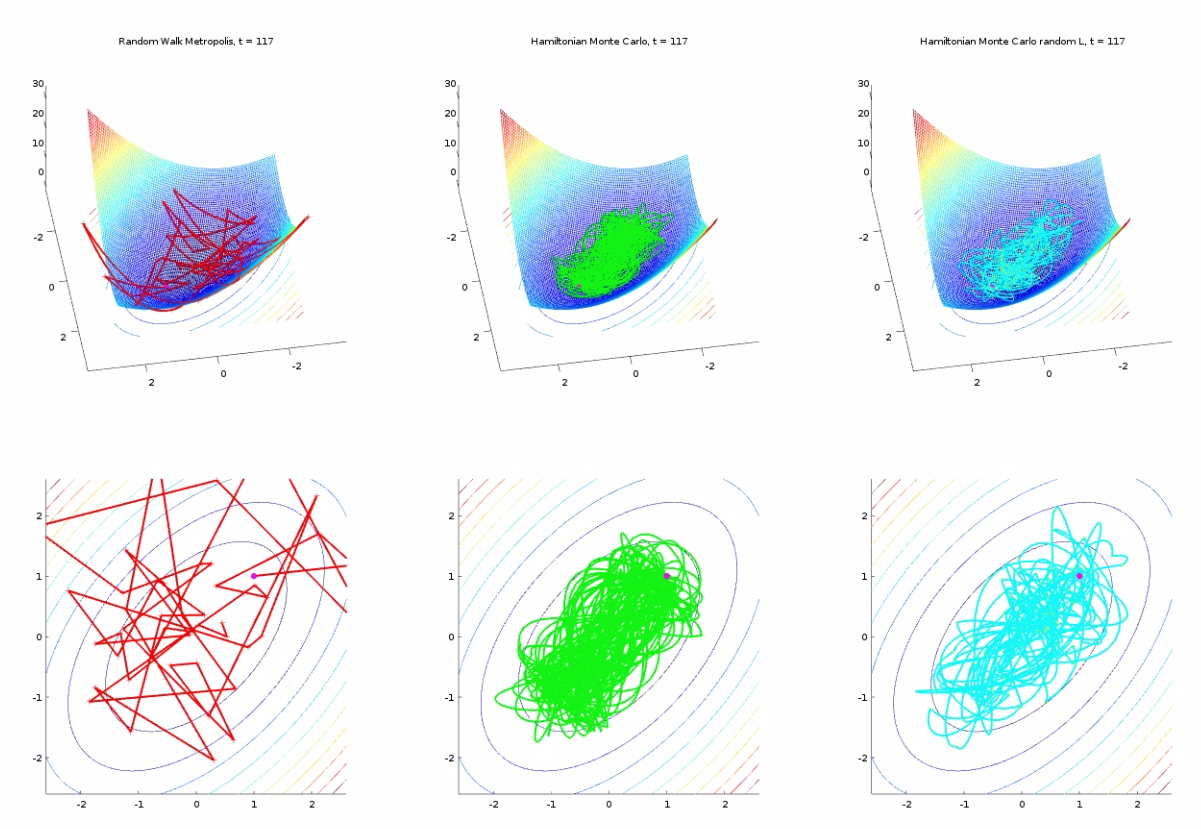
\includegraphics[width=0.8\textwidth]{figs/normal.png}
    \caption{$X_0 = (0,1)$ est proche du mode}  
  \end{subfigure}

  \begin{subfigure}{\textwidth}  
    \centering
    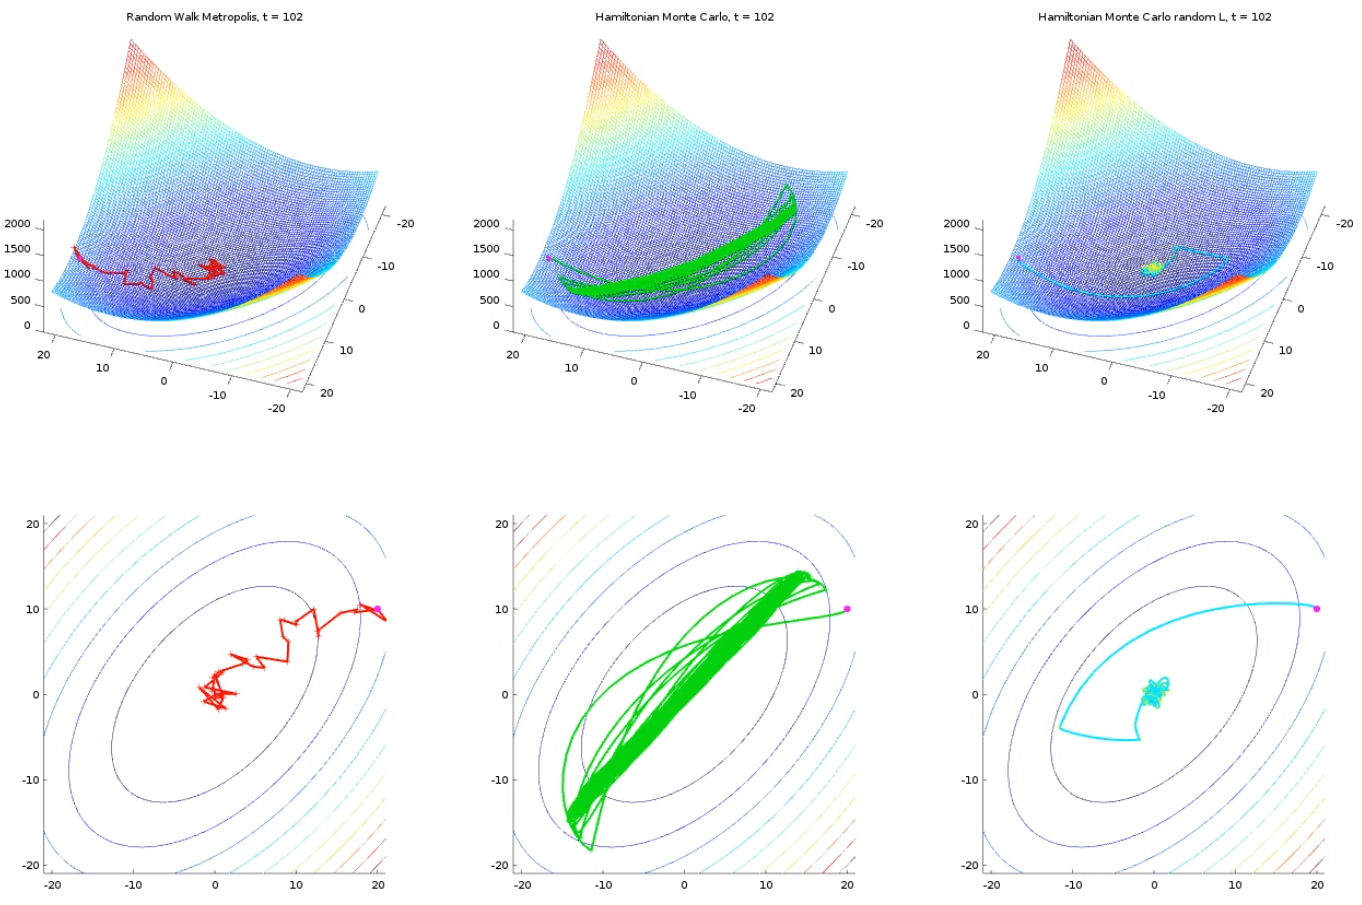
\includegraphics[width=0.8\textwidth]{figs/normal_far.png}
    \caption{$X_0 = (10, 20)$ est loin du mode}  
  \end{subfigure}
  \caption{Trajectoires sur loi normale. En rouge RWM, en vert HMC, en cyan HMC avec L aléatoire. La surface et les lignes de niveaux correspondent à $U$. \label{fig:normal}}
\end{figure}

\begin{figure}[ht]
  \centering
  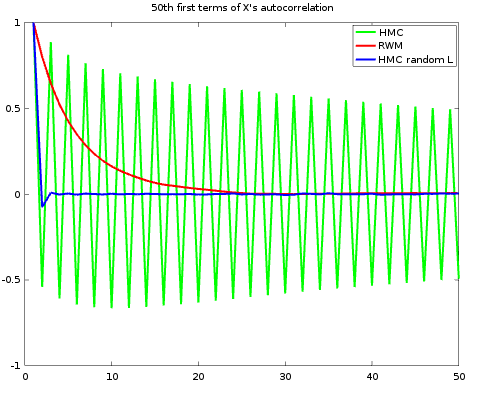
\includegraphics[width=0.5\textwidth]{figs/normal_autocor.png}
  \caption{Autocorrelations sur loi normale. \label{fig:normal_autocor}}
\end{figure}

\pagebreak
\subsection{Test sur un mélange de gaussiennes}
On considère ici $\pi = 0.8 \times \calN\left(\begin{bmatrix} 2 \\ 2 \end{bmatrix}, \begin{bmatrix}
0.5 & 0 \\ 0 & 0.5 \end{bmatrix}\right) + 0.2 \times \calN\left(\begin{bmatrix} -2 \\ -2 \end{bmatrix}, \begin{bmatrix} 0.5 & 0 \\ 0 & 0.5 \end{bmatrix}\right)$. Le point de départ est $X_0 = 0$. 

La figure \ref{fig:gm_autocor} montre le même comportement : des oscillations pour le HMC avec $L$ constant et autocorrelation plus faible pour le HMC avec $L$ aléatoire. Néanmoins, remarquons ici que le fait de prendre $L$ constant permet de visiter plus rapidement les deux creux de l'énergie potentielle. En effet, en environ $200$ itérations, seul le HMC avec $L$ constant arrive à sortir du creux le plus profond. Le fait d'avoir pris $L \sim \calU(\iseg{1,25})$ permet de réduire les mouvements et donc d'avoir une meilleure autocorrelation mais, si on effectue trop de petits mouvements, l'algorithme n'arrive pas à sortir du creux le plus profond (ce qui correspond au même comportement que le RWM). 

\begin{figure}[ht]
  \centering
  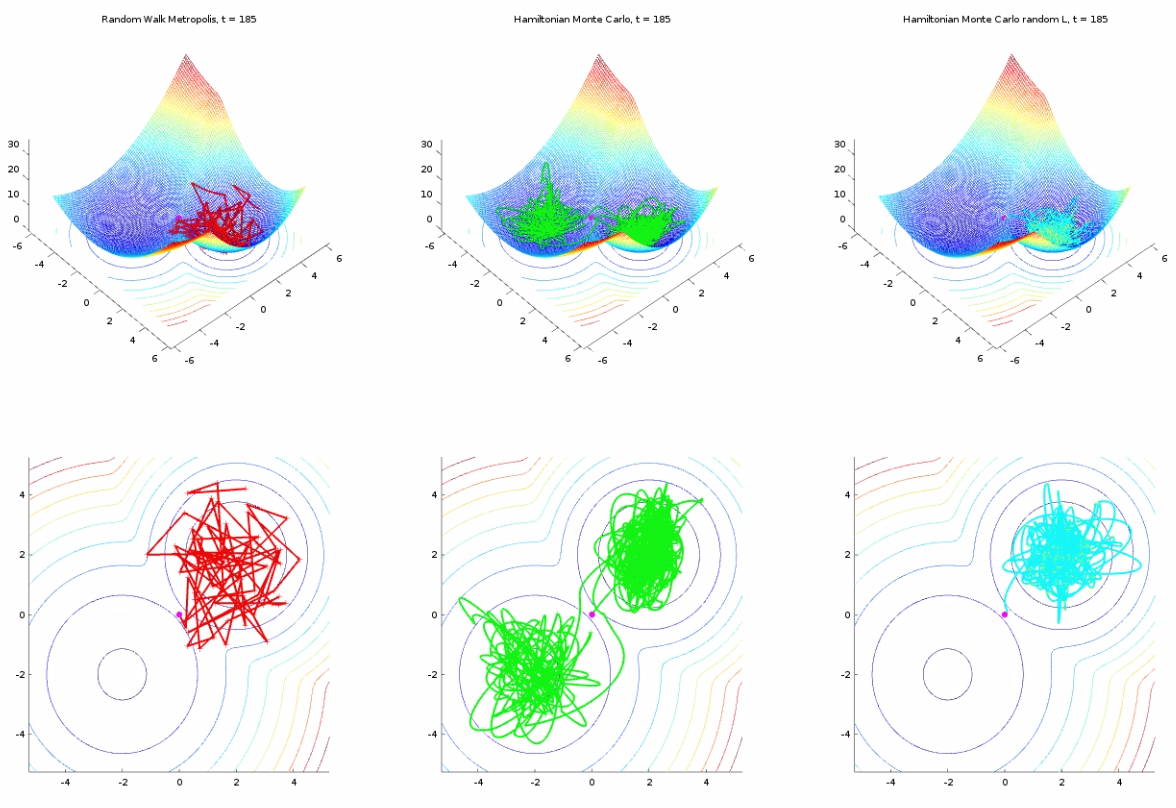
\includegraphics[width=0.8\textwidth]{figs/gm.png}
  \caption{Trajectoires sur mélange de gaussiennes. En rouge RWM, en vert HMC, en cyan HMC avec L aléatoire. La surface et les lignes de niveaux correspondent à $U$. \label{fig:gm}}
\end{figure}

\begin{figure}[ht]
  \centering
  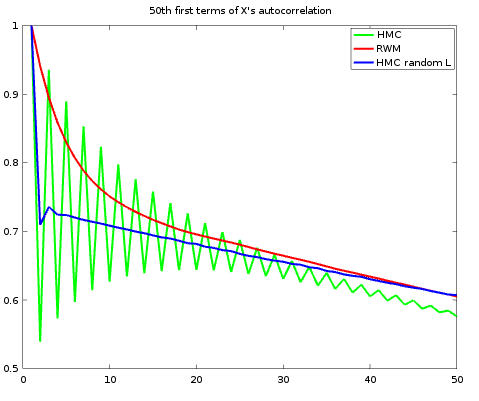
\includegraphics[width=0.5\textwidth]{figs/gm_autocor.png}
  \caption{Autocorrelations sur mélange de gaussiennes. \label{fig:gm_autocor}}
\end{figure}

\subsection{Test sur le bayesian lasso}
On considère ici $U(x) = \norm{Ax - b}_2^2 + \lambda \norm{x}_1$ qui n'est pas différentiable, ainsi au lieu de considérer le gradient de $U$, on considère la sous-différentielle $(A + A^\top) x + \lambda \sign(x)$. Dans les simulations, on prend $A = \begin{bmatrix} 0.5 & 0.4 \\ 0.5 & 0.4 \end{bmatrix}$, $b = \begin{bmatrix} 0.1 \\ 0.1 \end{bmatrix}$ et $\lambda = 2$.

D'après la figure \ref{fig:bl}, lorsque $X_0$ est proche du mode, les trois algorithmes semblent se comporter de manière correcte, similaire à la loi normale. Les autocorrelations (figure \ref{fig:bl_autocor}) semblent même être très bonnes pour les deux cas du HMC. Mais ce résultat est à considérer avec précaution. En effet, comme on le voit dans le cas où $X_0$ est loi du mode, dans les deux cas, l'algorithme HMC fait peu de mouvements (i.e il rejette très souvent le mouvement proposé). Ainsi il se peut que les bons résultats obtenus pour l'autocorrelation viennent du fait que l'algorithme reste souvent à la même position. 

\begin{figure}[hp]
  \begin{subfigure}{\textwidth}  
    \centering
    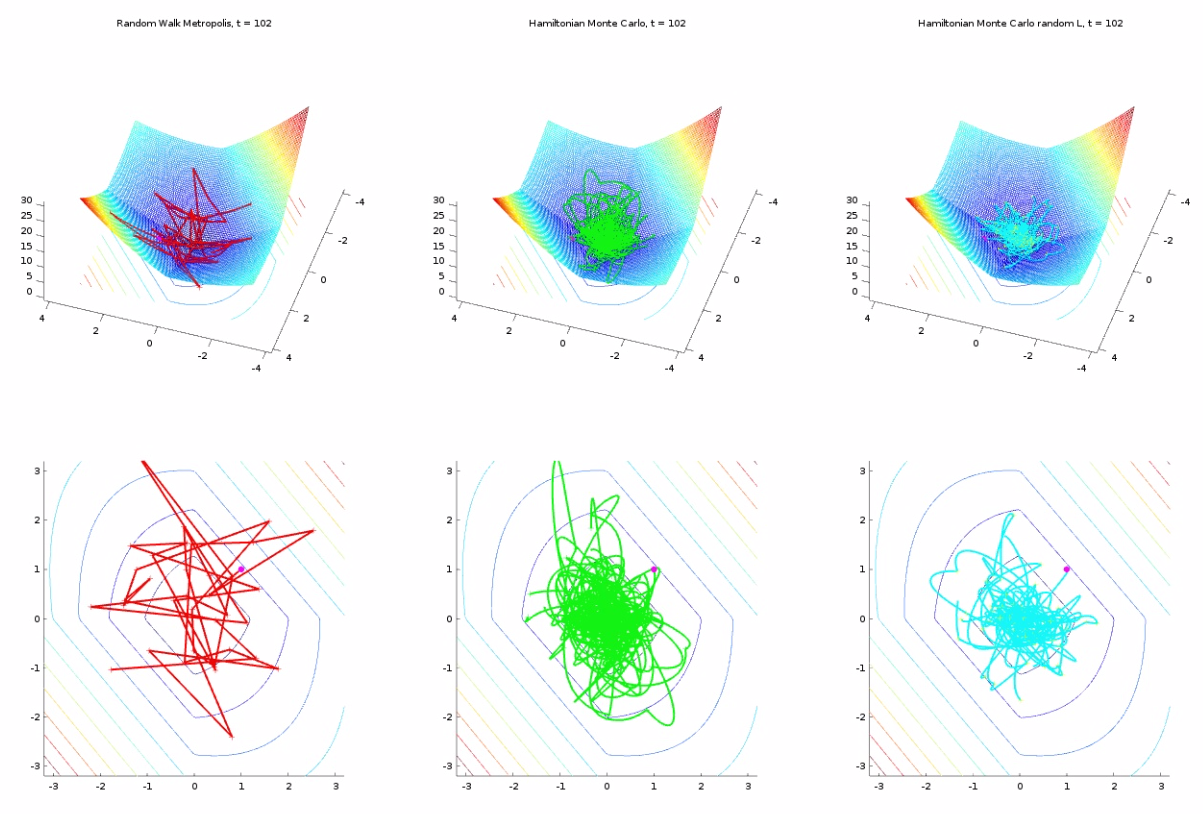
\includegraphics[width=0.8\textwidth]{figs/bl.png}
    \caption{$X_0 = (0,1)$ est proche du mode}  
  \end{subfigure}

  \begin{subfigure}{\textwidth}  
    \centering
    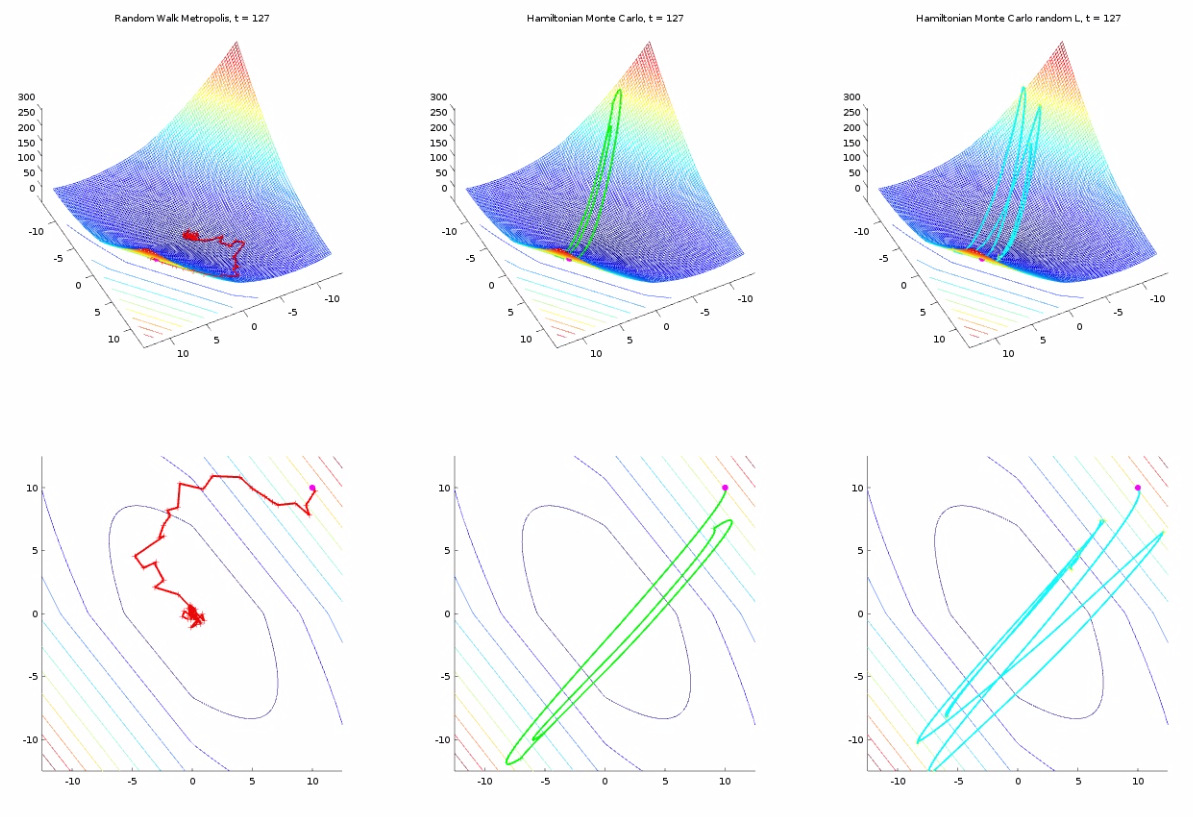
\includegraphics[width=0.8\textwidth]{figs/bl_far.png}
    \caption{$X_0 = (10, 10)$ est loin du mode}  
  \end{subfigure}
  \caption{Trajectoires sur bayesian lasso. En rouge RWM, en vert HMC, en cyan HMC avec L aléatoire. La surface et les lignes de niveaux correspondent à $U$. \label{fig:bl}}
\end{figure}

\begin{figure}[ht]
  \centering
  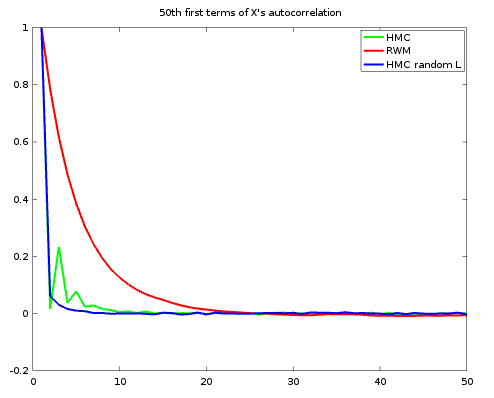
\includegraphics[width=0.5\textwidth]{figs/bl_autocor.png}
  \caption{Autocorrelations sur bayesian lasso. \label{fig:bl_autocor}}
\end{figure}

\section{Conclusion}
L'idée de base du Hamiltonian Monte Carlo est assez intuitive : plutôt que de considérer des mouvements de marche aléatoire (Random-walk Metropolis), il serait plus intéressant de proposer des mouvements qui prennent compte de la forme de la densité à simuler. Nous avons vu que l'algorithme proposé permet bien de générer une chaîne de Markov pour laquelle la loi cible est invariante à la fois dans le cas où l'on simule exactement la dynamique hamiltonienne et dans le cas où celle-ci est approchée (et où l'on insère alors le mouvement dans une stratégie Metropolis).

En pratique, nous avons vu que l'algorithme HMC tend à donner de meilleurs résultat que le RMW surtout lorsque la durée de la simulation {\it leapfrog} $L$ est tiré aléatoirement à chaque itération. Le paramètre $L$ semble influencer grandement les performances de l'algorithme. Neal \cite{Neal-hmc} mentionne le fait que choisir $L$ aléatoire permet d'éviter des effets de cycles dans le mouvement. Cette observation fait l'objet d'un contre exemple dans \cite{ergodicity-hmc} où les auteurs fournissent des hypothèses nécessaires sur la loi de $L$ afin d'obtenir l'ergodicité géométrique de l'algorithme HMC. Enfin, nous avons pu voir l'importance des hypothèses \eqref{eq:hyp} dans le cas du bayésian lasso où l'énergie potentielle n'est pas différentiable. La dynamique hamiltonienne n'étant pas bien simulée, l'algorithme HMC a tendance à refuser très souvent le mouvement. 

\pagebreak
\bibliographystyle{plain}
\bibliography{ref}
\end{document}


